\documentclass[11pt, english]{report}
\usepackage{graphicx}
\usepackage[colorlinks=true, linkcolor=blue]{hyperref}
\usepackage[english]{babel}
\selectlanguage{english}
\usepackage[utf8]{inputenc}
\usepackage[svgnames]{xcolor}
\usepackage{url}
\usepackage{hyperref}
\usepackage{float}
\usepackage{longtable}
\usepackage[toc]{glossaries}
\usepackage{amsmath}
\usepackage{amssymb}

\usepackage{algpseudocode}
\usepackage{algorithm}
\usepackage{csquotes}

\usepackage{listings}

\newcommand{\R}{\mathbb{R}}


\usepackage{listings}
\usepackage{afterpage}
\pagestyle{plain}


\definecolor{dkgreen}{rgb}{0,0.6,0}
\definecolor{gray}{rgb}{0.5,0.5,0.5}
\definecolor{mauve}{rgb}{0.58,0,0.82}
\usepackage{biblatex}
\bibliography{ref.bib}

%\lstset{language=R,
%    basicstyle=\small\ttfamily,
%   stringstyle=\color{DarkGreen},
%    otherkeywords={0,1,2,3,4,5,6,7,8,9},
%    morekeywords={TRUE,FALSE},
%    deletekeywords={data,frame,length,as,character},
%    keywordstyle=\color{blue},
%    commentstyle=\color{DarkGreen},
%}

\lstset{frame=tb,
language=R,
aboveskip=3mm,
belowskip=3mm,
showstringspaces=false,
columns=flexible,
numbers=none,
keywordstyle=\color{blue},
numberstyle=\tiny\color{gray},
commentstyle=\color{dkgreen},
stringstyle=\color{mauve},
breaklines=true,
breakatwhitespace=true,
tabsize=3
}


\usepackage{here}


\textheight=21cm
\textwidth=17cm
%\topmargin=-1cm
\oddsidemargin=0cm
\parindent=0mm
\pagestyle{plain}

\usepackage{color}
\usepackage{ragged2e}

\global\let\date\relax
\newcounter{unomenos}
\setcounter{unomenos}{\number\year}
\addtocounter{unomenos}{-1}
\stepcounter{unomenos}
\gdef\@date{ Course \arabic{unomenos}/ 2019}

\makeglossaries
 
\newglossaryentry{eternity}
{
    name=ETERNITY: FUNCTIONS,
    description={It stands for the name of both the project and the product, unless otherwise stated}
}

\begin{document}

\begin{titlepage}

\begin{center}
\vspace*{-1in}
\begin{figure}[htb]
\begin{center}

\includegraphics[width=8cm]{logo}
\end{center}
\end{figure}
\begin{Large}
\textbf{SOEN 6011 - Software Engineering Processes} \\
\end{Large}
\vspace*{0.1in}
Summer 2019\\
\vspace*{0.5in}
\begin{Large}
\textbf{Scientific Calculator-  ETERNITY: FUNCTIONS} \\
\end{Large}
\vspace*{0.4in}
\begin{large}
Project Report\\
\end{large}
\vspace*{0.2in}
\begin{Large}
\textbf{Deliverable 2} \\
\end{Large}
\vspace*{0.3in}
\begin{large}
Presented to \\
\vspace*{0.1in}
Instructor: PANKAJ KAMTHAN 
 \\
\end{large}
\vspace*{0.3in}
\rule{80mm}{0.1mm}\\
\vspace*{0.1in}
\begin{large}
By \\
Prashanthi Ramesh\\ 
\vspace*{0.3in}
\date{\normalsize\today} 

\end{large}
\end{center}
\end{titlepage}

\newcommand{\CC}{C\nolinebreak\hspace{-.05em}\raisebox{.4ex}{\tiny\bf +}\nolinebreak\hspace{-.10em}\raisebox{.4ex}{\tiny\bf +}}
\def\CC{{C\nolinebreak[4]\hspace{-.05em}\raisebox{.4ex}{\tiny\bf ++}}}

\tableofcontents
\newpage
\chapter{Changes}

\section{From Deliverable 1 to Deliverable 2}

\begin{enumerate}
    \item In deliverable 1, the requirement with ID= $EF\_REQ\_6$ states that $0^0=Error$ which is incorrect. The requirement is corrected as $0^0=1$ and the unit test cases are created accordingly.
    \item In deliverable 1, the requirement with ID= $EF\_REQ\_8$ states that zero raised to a real number is 1 which is incorrect. The requirement is corrected as $0^y=0$ where y is a real number and the unit test cases are created accordingly.
    \item In deliverable 2 there is an addition of a new algorithm to calculate the power of non-fractional number by the method of squaring. The fractional part uses the pseudo-code mentioned in deliverable 1 which is bit manipulation approximation method.
\end{enumerate}

\chapter{Problem 4}

This section presents an overview of the source code of the Eternity Function application and the practices followed during the development.

\section{Programming Style of Source Code}

We collaboratively as a team brainstormed and decided to follow the Google Java Style\cite{googlestyle} programming style. 

\subsection{Google Java Style- Benefits}

The benefits are as follows:

\begin{itemize}
    \item Compatible with popular IDE (Integrated Development Environment) like Eclipse and IntelliJ IDEA.
    \item The style checker will automatically highlight any deviations from the code standards as we write code.
\end{itemize} 

\section{User Interface Design Pattern}

\subsection{Memento Design Pattern}

\begin{figure}[H]
  
  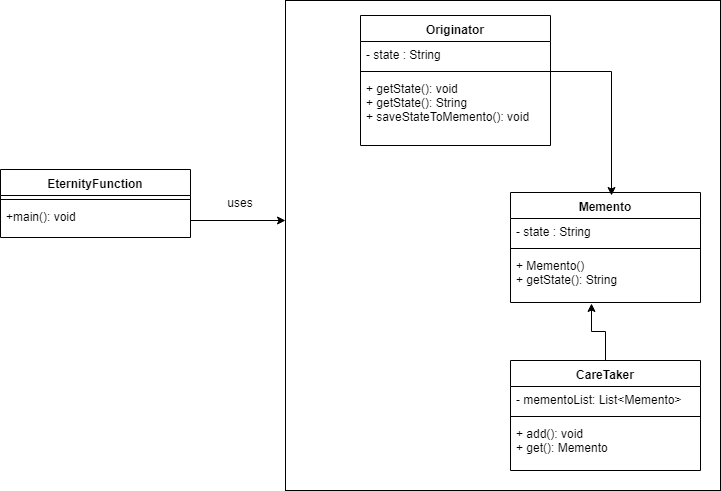
\includegraphics[width=1\textwidth]{memento.png}
  \centering
  \caption{The Memento Design pattern UML diagram representation
}
\end{figure}

The memento design pattern\cite{memento} is implemented in the Eternity Function to maintain a list of all previous operation that it has performed.\\

Hence, the user of the Eternity Function would be able to restore a previous calculation performed.\\

The use of memento design pattern prevents the EternityFunction object from becoming large and complex.\\

\begin{figure}[H]
  
  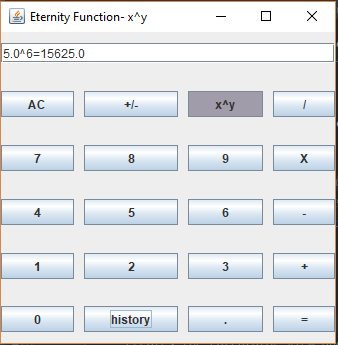
\includegraphics[width=0.6\textwidth]{d2.PNG}
  \centering
  \caption{The history of operations of Eternity Function implemented using memento design pattern
}
\end{figure}

\section{Error Handling}

When an exception occurs in Eternity Function, we say that the exception is "thrown."  \\

Double.parseDouble(textFieldValue) throws an exception of type NumberFormatException when the value entered in the text field is any character other than real numbers. \\

When an exception is thrown, it is possible to "catch" the exception and prevent it from crashing the program. This is done with a try..catch statement in Eternity Function. \\

In simplified form, the syntax for a try..catch statement can be:

\begin{lstlisting}
try {
   statements-1
   ...
   Double.parseDouble(textFieldValue)
   ...
}
catch ( NumberFormatException exception) {
   statements-2
}
\end{lstlisting}

\begin{figure}[H]
  
  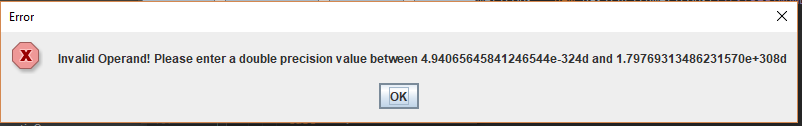
\includegraphics[width=1\textwidth]{d2p2.PNG}
  \centering
  \caption{ An Error message in the EternityFunction that aims to be helpful
}
\end{figure}

\begin{figure}[H]
  
  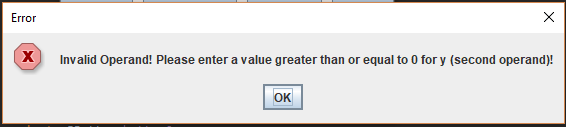
\includegraphics[width=1\textwidth]{d2p4.PNG}
  \centering
  \caption{ Another instance of an error message in the EternityFunction that aims to be helpful
}
\end{figure}

\section{Debugger}

IntelliJ IDEA build-in debugger is used for debugging the Eternity Function application. \\

\begin{itemize}
    \item The IntelliJ IDEA debugger offers a rich experience that helps us to easily debug anything from the simplest code to complex multi-threaded applications.
    \item Smart Step Into action allows to skip all intermediate invocations and proceed to the target method directly.
    \item IntelliJ allows creating breakpoints that pause the execution only if a user-defined condition is satisfied.
    \item IntelliJ allows to attach custom labels to JVM objects.
    \item An object can be marked when an application is stopped on a breakpoint and the target is reachable from stack frames.
\end{itemize}


\setlength{\tabcolsep}{18pt}
\renewcommand{\arraystretch}{1.5}
\begin{tabular}{ |p{6cm}|p{6cm}| }
\hline
\textbf{Advantages} & \textbf{Disadvantages}\\ \hline 
If we don't have the source to specific code, IntelliJ IDEA will still decompile the class and show our steps in the decompiled source.
 & Code that was compiled without the debug flag cannot be debugged.\\
\hline
we can define in IntelliJ IDEA a breakpoint to stop before entry or exit from a specific method, even if the method itself was compiled without the debug flag & Line breakpoints are also not possible to define and hit.\\
\hline
The Remove Once Hit option is a very useful feature and its use is as a filter to triggering a breakpoint in a scenario where we're interested in a visit to a method, or a specific state in the code only after another state was reached.  & Method Breakpoint and Field Watchpoint slow down code execution considerably.\\
\hline
If we stepped too far and want to go back up the stack to then re-execute the code, we can use the Drop Frame feature. & Drop Frame feature is also potentially dangerous: we must be aware that re-executing the code will execute the same instructions twice, and if those instructions modify state we might end up in a corrupted state.\\
\hline
\end{tabular} \\ \\ \\ 

\section{Quality Attributes}

\subsection{Correct}

\begin{itemize}
    \item The Eternity Function application code is in agreement with specifications
    \item The correctness of the application is verified by unit testing using JUnit.
    \item Unit testing is used to ensure that the program quality standards are met and that the program is correct.
\end{itemize}

\begin{figure}[H]
  
  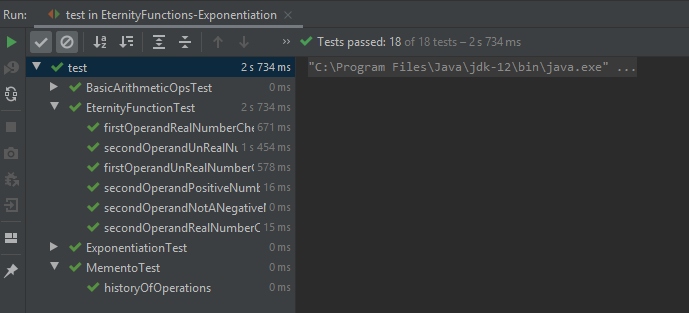
\includegraphics[width=1\textwidth]{d2p5.PNG}
  \centering
  \caption{A success run of the JUnit test cases
}
\end{figure}

\subsection{Efficient}

\begin{itemize}
    \item The use of approximation algorithms\cite{power} which are efficient algorithms makes Eternity Function efficient.
    \item Since the exponentiation routines of typical math libraries are rather slow, their replacement with a fast approximation can greatly reduce the overall computation time.
    \item An approximation is perfectly adequate for most neural computation purposes and can save much time.
    \item This approximation method is about 20 times as fast as Math.pow().
\end{itemize}

\subsection{Maintainable}

\begin{itemize}
    \item The use of memento design provide easier maintainability and reusability,
more understandable implementation and more flexible
design.
    \item Writing comments and Javadoc increases understand-ability of code and thus makes it easier to be maintained.
\end{itemize}

\subsection{Robust}

\begin{itemize}
    \item Eternity Function can cope with errors during execution.
    \item Robustness is achieved by using exception handlers.
\end{itemize}

\subsection{Usable}

\begin{itemize}
    \item The Eternity Function shall be used by members of public without training.
    \item The Eternity Function user interface design is clear and easy to understand
\end{itemize}

\section{Quality Checker}

To check the quality of the Eternity Functions's source code, Checkstyle\cite{checkstyle} tool is used. This section presents an overview of Checkstyle tool.

\subsection{Checkstyle}

\begin{itemize}
    \item Checkstyle is a development tool to help programmers write Java code that adheres to a coding standard.
    \item It automates the process of checking Java code to spare humans of this boring (but important) task.
    \item This makes it ideal for projects that want to enforce a coding standard.
    \item Checkstyle is highly configurable and can be made to support almost any coding standard.
    \item It can find class design problems, method design problems. 
    \item It also has the ability to check code layout and formatting issues.
\end{itemize}

\begin{figure}[H]
  
  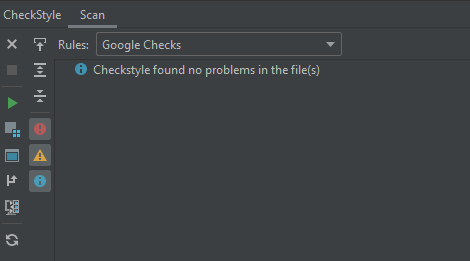
\includegraphics[width=1\textwidth]{d2p3.PNG}
  \centering
  \caption{ The google checkstyle validates that the quality of the source code is good 
}
\end{figure}

\setlength{\tabcolsep}{18pt}
\renewcommand{\arraystretch}{1.5}
\begin{tabular}{ |p{6cm}|p{6cm}| }
\hline
\textbf{Advantages} & \textbf{Disadvantages}\\ \hline 
Portable between IDEs. If you decide to use IntelliJ later, or you have a team using a variety of IDEs, you still have a way to enforce consistency.
 & It is not in-build with IDE's and needs to be configured manually.\\
\hline
better external tooling. It's much easier to integrate checkstyle with your external tools since it was really designed as a standalone framework. & With a bad configuration, you may check things twice or two opposite things i.e "Remove useless constructors" and "Always one constructor".\\
\hline
ability of creating your own rules. IDE defines a large set of styles, but checkstyle has more, and you can add your own custom rules.  & Is not used for checking more complicate rules like during the design of your classes, or for more special problems like implementing correctly the clone function. \\
\hline
If we stepped too far and want to go back up the stack to then re-execute the code, we can use the Drop Frame feature. & Drop Frame feature is also potentially dangerous: we must be aware that re-executing the code will execute the same instructions twice, and if those instructions modify state we might end up in a corrupted state.\\
\hline
\end{tabular} \\ \\ \\ 

\chapter{Problem 6}

\section{Unit Test Cases}

This section presents the unit test cases implemented using JUnit for Eternity Function which are traceable to requirements. \\ \\

\setlength{\tabcolsep}{18pt}
\renewcommand{\arraystretch}{1.5}
\begin{tabular}{ |p{4cm}|p{8cm}| }
\hline
\textbf{Test Case ID} & EF\_TESTCASE\_1 \\ \hline 
\textbf{Requirement ID} & EF\_REQ\_4, EF\_REQ\_5\\ \hline
\textbf{Action} & The user enters input in the text field and clicks a button \\ \hline
\textbf{Input(s)} & first operand is 563248.2656E and operator is $\wedge$  \\ \hline
\textbf{Expected Output} & isFirstNotRealNumber() returns true \\ \hline
\textbf{Actual Output} & isFirstNotRealNumber() returns true \\ \hline
\textbf{Test Result} & Success \\ 
\hline
\end{tabular} \\ \\ \\

\setlength{\tabcolsep}{18pt}
\renewcommand{\arraystretch}{1.5}
\begin{tabular}{ |p{4cm}|p{8cm}| }
\hline
\textbf{Test Case ID} &  EF\_TESTCASE\_2 \\ \hline 
\textbf{Requirement ID} & EF\_REQ\_3\\ \hline
\textbf{Action} & The user enters input in the text field and clicks a button \\ \hline
\textbf{Input(s)} & first operand is 563248.2656 and operator is $\wedge$  \\ \hline
\textbf{Expected Output} & isFirstNotRealNumber() returns false \\ \hline
\textbf{Actual Output} & isFirstNotRealNumber() returns false \\ \hline 
\textbf{Test Result} & Success \\ 
\hline
\end{tabular} \\ \\ \\

\setlength{\tabcolsep}{18pt}
\renewcommand{\arraystretch}{1.5}
\begin{tabular}{ |p{2.2cm}|p{9.8cm}| }
\hline
\textbf{Test Case ID} & EF\_TESTCASE\_3 \\ \hline 
\textbf{Requirement ID} & EF\_REQ\_4\\ \hline
\textbf{Action} & The user enters input in the text field and clicks a button and enters another value in the text field\\ \hline
\textbf{Input(s)} & first operand is 563248.2656 and operator is $\wedge$ and second operand is 6526.25654 \\ \hline
\textbf{Expected Output} & isSecondNotRealNumber() returns false \\ \hline
\textbf{Actual Output} & isSecondNotRealNumber() returns false \\ \hline
\textbf{Test Result} & Success \\ 
\hline
\end{tabular} \\ \\ \\

\setlength{\tabcolsep}{18pt}
\renewcommand{\arraystretch}{1.5}
\begin{tabular}{ |p{4cm}|p{8cm}| }
\hline
\textbf{Test Case ID} &  EF\_TESTCASE\_4 \\ \hline 
\textbf{Requirement ID} & EF\_REQ\_3, EF\_REQ\_5\\ \hline
\textbf{Action} & The user enters input in the text field and clicks a button and enters another value in the text field\\ \hline
\textbf{Input(s)} & first operand is 563248.2656 and operator is $\wedge$ and second operand is 6526.25654E \\ \hline
\textbf{Expected Output} & isSecondNotRealNumber() returns true \\ \hline
\textbf{Actual Output} & isSecondNotRealNumber() returns true \\ \hline
\textbf{Test Result} & Success \\ 
\hline
\end{tabular} \\ \\ \\

\setlength{\tabcolsep}{18pt}
\renewcommand{\arraystretch}{1.5}
\begin{tabular}{ |p{4cm}|p{8cm}| }
\hline
\textbf{Test Case ID} &  EF\_TESTCASE\_5 \\ \hline 
\textbf{Requirement ID} & EF\_REQ\_7\\ \hline
\textbf{Action} & The user enters input in the text field and clicks a button and enters another value in the text field\\ \hline
\textbf{Inputs} & first operand is 563248.2656 and operator is $\wedge$ and second operand is -543543.43432 \\ \hline
\textbf{Expected Output} & isaNegativeValue() returns true \\ \hline
\textbf{Actual Output} & isaNegativeValue() returns true \\ \hline
\textbf{Test Result} & Success \\ 
\hline
\end{tabular} \\ \\ \\

\setlength{\tabcolsep}{18pt}
\renewcommand{\arraystretch}{1.5}
\begin{tabular}{ |p{4cm}|p{8cm}| }
\hline
\textbf{Test Case ID} &  EF\_TESTCASE\_6 \\ \hline 
\textbf{Requirement ID} & EF\_REQ\_7\\ \hline
\textbf{Action} & The user enters input in the text field and clicks a button and enters another value in the text field\\ \hline
\textbf{Input(s)} & first operand is 563248.2656 and operator is $\wedge$ and second operand is -543543.43432 \\ \hline
\textbf{Expected Output} & isaNegativeValue() returns false \\ \hline
\textbf{Actual Output} & isaNegativeValue() returns false \\ \hline
\textbf{Test Result} & Success \\ 
\hline
\end{tabular} \\ \\ \\

\setlength{\tabcolsep}{18pt}
\renewcommand{\arraystretch}{1.5}
\begin{tabular}{ |p{4cm}|p{8cm}| }
\hline
\textbf{Test Case ID} &  EF\_TESTCASE\_7 \\ \hline 
\textbf{Requirement ID} & EF\_REQ\_1\\ \hline
\textbf{Action} & The user enters input in the text field and clicks a button and enters another value in the text field\\ \hline
\textbf{Input(s)} & first operand is 5.698468 and operator is $\wedge$ and second operand is 0 \\ \hline
\textbf{Expected Output} & exponentiation.power() returns 1 \\ \hline
\textbf{Actual Output} & exponentiation.power() returns 1 \\ \hline
\textbf{Test Result} & Success \\ 
\hline
\end{tabular} \\ \\ \\

\setlength{\tabcolsep}{18pt}
\renewcommand{\arraystretch}{1.5}
\begin{tabular}{ |p{4cm}|p{8cm}| }
\hline
\textbf{Test Case ID} &  EF\_TESTCASE\_8 \\ \hline 
\textbf{Requirement ID} & EF\_REQ\_2\\ \hline
\textbf{Action} & The user enters input in the text field and clicks a button and enters another value in the text field\\ \hline
\textbf{Input(s)} & first operand is 72645.3625892 and operator is $\wedge$ and second operand is 1 \\ \hline
\textbf{Expected Output} & exponentiation.power() returns 72645.3625892 \\ \hline
\textbf{Actual Output} & exponentiation.power() returns 72645.3625892 \\ \hline
\textbf{Test Result} & Success \\ 
\hline
\end{tabular} \\ \\ \\

\setlength{\tabcolsep}{18pt}
\renewcommand{\arraystretch}{1.5}
\begin{tabular}{ |p{4cm}|p{8cm}| }
\hline
\textbf{Test Case ID} &  EF\_TESTCASE\_9 \\ \hline 
\textbf{Requirement ID} & EF\_REQ\_6\\ \hline
\textbf{Action} & The user enters input in the text field and clicks a button and enters another value in the text field\\ \hline
\textbf{Input(s)} & first operand is 0 and operator is $\wedge$ and second operand is 0 \\ \hline
\textbf{Expected Output} & exponentiation.power() returns 1 \\ \hline
\textbf{Actual Output} & exponentiation.power() returns 1 \\ \hline
\textbf{Test Result} & Success \\ 
\hline
\end{tabular} \\ \\ \\

\setlength{\tabcolsep}{18pt}
\renewcommand{\arraystretch}{1.5}
\begin{tabular}{ |p{4cm}|p{8cm}| }
\hline
\textbf{Test Case ID} &  EF\_TESTCASE\_10 \\ \hline 
\textbf{Requirement ID} & EF\_REQ\_8\\ \hline
\textbf{Action} & The user enters input in the text field and clicks a button and enters another value in the text field\\ \hline
\textbf{Input(s)} & first operand is 0 and operator is $\wedge$ and second operand is 856954745.2545523 \\ \hline
\textbf{Expected Output} & exponentiation.power() returns 0 \\ \hline
\textbf{Actual Output} & exponentiation.power() returns 0 \\ \hline
\textbf{Test Result} & Success \\ 
\hline
\end{tabular} \\ \\ \\

\setlength{\tabcolsep}{18pt}
\renewcommand{\arraystretch}{1.5}
\begin{tabular}{ |p{4cm}|p{8cm}| }
\hline
\textbf{Test Case ID} &  EF\_TESTCASE\_11 \\ \hline 
\textbf{Requirement ID} & EF\_REQ\_9\\ \hline
\textbf{Action} & The user enters input in the text field and clicks a button and enters another value in the text field\\ \hline
\textbf{Input(s)} & first operand is -4 and operator is $\wedge$ and second operand is 7 \\ \hline
\textbf{Expected Output} & exponentiation.power() returns -16384 \\ \hline
\textbf{Actual Output} & exponentiation.power() returns -16384 \\ \hline
\textbf{Test Result} & Success \\ 
\hline
\end{tabular} \\ \\ \\

\setlength{\tabcolsep}{18pt}
\renewcommand{\arraystretch}{1.5}
\begin{tabular}{ |p{4cm}|p{8cm}| }
\hline
\textbf{Test Case ID} &  EF\_TESTCASE\_12 \\ \hline 
\textbf{Requirement ID} & EF\_REQ\_10\\ \hline
\textbf{Action} & The user enters input in the text field and clicks a button and enters another value in the text field\\ \hline
\textbf{Input(s)} & first operand is -4 and operator is $\wedge$ and second operand is 8 \\ \hline
\textbf{Expected Output} & exponentiation.power() returns 65536 \\ \hline
\textbf{Actual Output} & exponentiation.power() returns 65536 \\ \hline
\textbf{Test Result} & Success \\ 
\hline
\end{tabular} \\ \\ \\

\setlength{\tabcolsep}{18pt}
\renewcommand{\arraystretch}{1.5}
\begin{tabular}{ |p{4cm}|p{8cm}| }
\hline
\textbf{Test Case ID} &  EF\_TESTCASE\_13 \\ \hline 
\textbf{Requirement ID} & EF\_REQ\_15\\ \hline
\textbf{Action} & The user clicks the history button\\ \hline
\textbf{Input(s)} & History of operations \\ \hline
\textbf{Expected Output} & originator.getState() returns previous saved operation \\ \hline
\textbf{Actual Output} & originator.getState() returns previous saved operation \\ \hline
\textbf{Test Result} & Success \\ 
\hline
\end{tabular} \\ \\ \\

\section{JUnit Standard Guidelines}

The guidelines to create unit test cases of high-quality are:

\begin{itemize}
    \item Did not use the test-case constructor to set up a test case
    \item Use of setUp() and tearDown() methods to initialize and release object resources
    \item Test case method names are meaningful
    \item Test cases are time-independent, small and fast
    \item Documented tests in javadoc
   
\end{itemize}

\appendix
\chapter{GitHub}
\section{Individual GitHub Link}
https://github.com/PrashanthiRamesh/SOEN-6011-Project-Calculator/

\section{Team GitHub Link}
https://github.com/niravjdn/SOEN-6011-Project/


\printbibliography

\printglossary

\end{document}